\documentclass[10pt]{article}
\usepackage[letterpaper]{geometry}
\geometry{verbose,tmargin=1in,bmargin=1in,lmargin=1in,rmargin=1in}
\usepackage{setspace}
\usepackage{ragged2e}
\usepackage{color}
\usepackage{titlesec}
\usepackage{graphicx}
\usepackage{float}
\usepackage{mathtools}
\usepackage{amsmath}
\usepackage[font=small,labelfont=bf,labelsep=period]{caption}
\usepackage[english]{babel}
\usepackage{indentfirst}
\usepackage{array}
\usepackage{makecell}
\usepackage[usenames,dvipsnames]{xcolor}
\usepackage{multirow}
\usepackage{tabularx}
\usepackage{arydshln}
\usepackage{caption}
\usepackage{subcaption}
\usepackage{xfrac}
\usepackage{etoolbox}
\usepackage{cite}
\usepackage{url}
\usepackage{dcolumn}
\usepackage{hyperref}
\usepackage{courier}
\usepackage{esvect}
\usepackage{commath}
\usepackage{verbatim} % for block comments
\usepackage{enumitem}
\usepackage{hyperref} % for clickable table of contents
\usepackage{braket}
\usepackage{titlesec}
\usepackage{booktabs}
\usepackage{gensymb}
\usepackage{listings}
\usepackage{cancel}
\usepackage[mathscr]{euscript}
\lstset{
    frame=single,
    	basicstyle=\ttfamily\small,
    breaklines=true,
    postbreak=\raisebox{0ex}[0ex][0ex]{\ensuremath{\color{red}\hookrightarrow\space}}
}

% for circled numbers
\usepackage{tikz}
\newcommand*\circled[1]{\tikz[baseline=(char.base)]{
            \node[shape=circle,draw,inner sep=2pt] (char) {#1};}}

\newcommand{\beq}{\begin{equation}}
\newcommand{\eeq}{\end{equation}}
\newcommand{\beqa}{\begin{equation}\begin{aligned}}
\newcommand{\eeqa}{\end{aligned}\end{equation}}

\titleclass{\subsubsubsection}{straight}[\subsection]

% define new command for triple sub sections
\newcounter{subsubsubsection}[subsubsection]
\renewcommand\thesubsubsubsection{\thesubsubsection.\arabic{subsubsubsection}}
\renewcommand\theparagraph{\thesubsubsubsection.\arabic{paragraph}} % optional; useful if paragraphs are to be numbered

\titleformat{\subsubsubsection}
  {\normalfont\normalsize\bfseries}{\thesubsubsubsection}{1em}{}
\titlespacing*{\subsubsubsection}
{0pt}{3.25ex plus 1ex minus .2ex}{1.5ex plus .2ex}

\makeatletter
\renewcommand\paragraph{\@startsection{paragraph}{5}{\z@}%
  {3.25ex \@plus1ex \@minus.2ex}%
  {-1em}%
  {\normalfont\normalsize\bfseries}}
\renewcommand\subparagraph{\@startsection{subparagraph}{6}{\parindent}%
  {3.25ex \@plus1ex \@minus .2ex}%
  {-1em}%
  {\normalfont\normalsize\bfseries}}
\def\toclevel@subsubsubsection{4}
\def\toclevel@paragraph{5}
\def\toclevel@paragraph{6}
\def\l@subsubsubsection{\@dottedtocline{4}{7em}{4em}}
\def\l@paragraph{\@dottedtocline{5}{10em}{5em}}
\def\l@subparagraph{\@dottedtocline{6}{14em}{6em}}
\makeatother


\setcounter{secnumdepth}{4}
\setcounter{tocdepth}{4}
\begin{document}

\title{MATH 228b: HW7}
\author{April Novak}

\maketitle

\section{(a)}
The {\tt euler\_fluxes.m} function returns the Euler fluxes \(F\) given inputs of the four conserved variables - density, two components of momentum, and total energy.

\section{(b)}
The {\tt spectral\_divergence.m} function calculates the divergence of a grid function using the FFT. Given a function \(v(x)\), first \(\hat{v}\) is computed, where \(\hat{v}\) is the Fourier transform of \(v\). Then, because the derivative of a Fourier transform is simply equal to the Fourier transform multiplied by \(ik\), where \(k\) are the discrete frequencies, the derivative in the Fourier transform space can be computed as \(\hat{w}=ik\hat{v}\). Finally, an inverse Fourier transform is performed to obtained \(w\), where \(w\) is the derivative of \(v\). This is the approach used to compute the divergence of a grid function. Note that this function only works for periodic grid functions - otherwise, the divergence ``blows up,'' especially near the domain boundaries.

\section{(c)}
Similar to the use of the Bubnov-Galerkin formulation for convection-diffusion problems, stabilization is required for spectral methods. This is achieved by using a filter, which essentially filters the grid solution by damping out high frequencies by multiplying low frequencies by a number very close to 1.0 and high frequencies by numbers close to 0.0. This is not a conservative method. The spectral filter is implemented by first filtering in the \(x\) direction, and then using this semi-filtered result as input for filtering in the \(y\) direction.

\section{(d)}
The right-hand side of the Euler equations (the divergence of the flux vector) is computed using {\tt euler\_rhs.m} by calling {\tt euler\_fluxes} followed by {\tt spectral\_divergence} once for each of the four equations present.

\section{(e)}
Given an initial condition from the {\tt euler\_vortex.m} function, {\tt euler\_rk4step} steps the solutions once using the RK-4 time stepping method and applies filtering to all solution components.

\section{(f)}
Fig. \ref{fig:convergence} shows the infinity norm errors as a function of the grid spacing \(h\) for the four solution components for the Euler vortex. As can be seen, spectral convergence is obtained, since the rate of convergence is not constant as a function of \(h\), but rather dramatically increases as \(h\) is refined. Fig. \ref{fig:100dt} shows the solution at 1.5615 seconds for \(N=32\). The code used to perform this convergence test is shown in {\tt script.m} in the Appendix.

\begin{figure}[H]
\centering
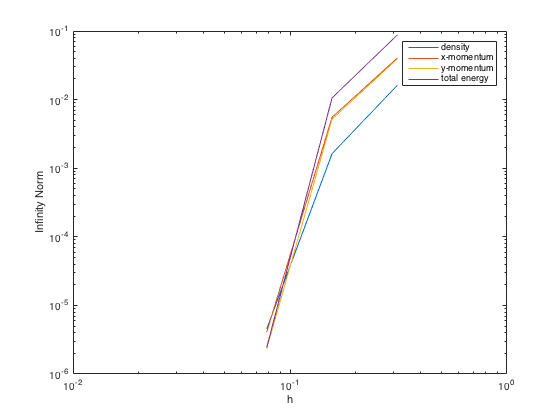
\includegraphics[width=0.8\textwidth]{figures/convergence.png}
\caption{Infinity norm as a function of mesh spacing \(h\) for the four solution components.}
\label{fig:convergence}
\end{figure}

\begin{figure}[H]
\centering
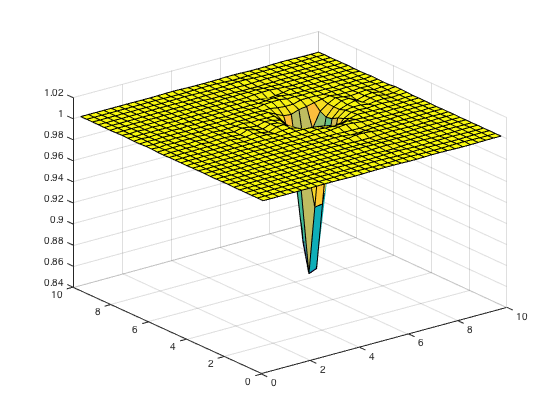
\includegraphics[width=0.8\textwidth]{figures/100dt.png}
\caption{Solution for \(N=32\) at \(t=1.5615\).}
\label{fig:100dt}
\end{figure}

\section{(g)}
Fig. \ref{fig:kh} shows the Kelvin-Helmholtz instability at 2 seconds, where the maximum and minimum values of \(\rho\) are 2.3312 and 0.5243, respectively. The script developed for this section is shown in the Appendix as {\tt kh.m}.

\begin{figure}[H]
\centering
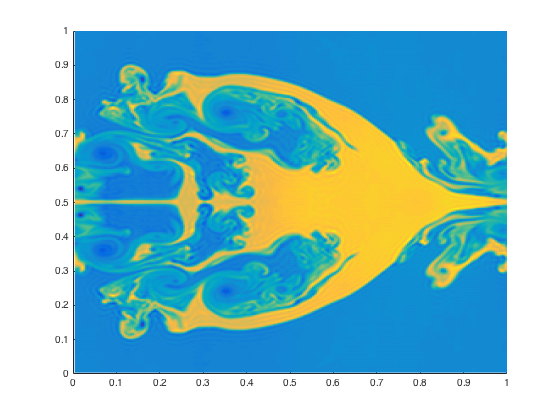
\includegraphics[width=0.8\textwidth]{figures/kh.png}
\caption{Density solution to the Kelvin-Helmholtz instability at 2 seconds.}
\label{fig:kh}
\end{figure}




\section{Appendix}
\subsection{{\tt euler\_fluxes.m}}
\lstinputlisting[language=Matlab]{euler_fluxes.m}
\subsection{{\tt spectral\_divergence.m}}
\lstinputlisting[language=Matlab]{spectral_divergence.m}
\subsection{{\tt spectral\_filter.m}}
\lstinputlisting[language=Matlab]{spectral_filter.m}
\subsection{{\tt euler\_rhs.m}}
\lstinputlisting[language=Matlab]{euler_rhs.m}
\subsection{{\tt euler\_rk4step.m}}
\lstinputlisting[language=Matlab]{euler_rk4step.m}
\subsection{{\tt script.m}}
\lstinputlisting[language=Matlab]{script.m}
\subsection{{\tt kh.m}}
\lstinputlisting[language=Matlab]{kh.m}

\end{document}
